\documentclass{article}

\usepackage{amsmath}
\usepackage{amsfonts}
\usepackage{tikz}
\usetikzlibrary{automata, positioning}

\title{$M/M/1/K$ Queue Analysis}
\author{Farbod Shahinfar}


\begin{document}
\maketitle{}

Consider a queue receiving requests with exponential (memory-less)
inter-arrival distribution and exponential service time. There is only one
service node and the maximum buffer size is $K$. This system is represented
with $M/M/1/K$ Kendall's notation. The request are either received and placed
in the queue or they are blocked. If the request are received, then they will
not live the queue until they are serviced. In this post, a basic analysis of
the system is performed.


\section{Stationary Probabilities of $M/M/1/K$}

\begin{figure}[!ht]
\centering
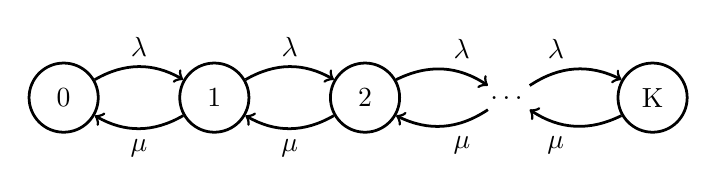
\begin{tikzpicture}[line width=1pt]
	\node[state] (q0) {0};
	\node[state, right= of q0] (q1) {1};
	\node[state, right= of q1] (q2) {2};
	\node[right= of q2] (dots) {\dots};
	\node[state, right= of dots] (qK) {K};
	\draw[->]
	(q0) edge[auto, bend left] node{$\lambda$} (q1)
	(q1) edge[auto, bend left] node{$\mu$} (q0)
	(q1) edge[auto, bend left] node{$\lambda$} (q2)
	(q2) edge[auto, bend left] node{$\mu$} (q1)
	(q2) edge[auto, bend left] node{$\lambda$} (dots)
	(dots) edge[auto, bend left] node{$\mu$} (q2)
	(dots) edge[auto, bend left] node{$\lambda$} (qK)
	(qK) edge[auto, bend left] node{$\mu$} (dots)
	;
\end{tikzpicture}
	\caption{This CTMC shows different states of $M/M/1/K$ system and transition rates.}
\end{figure}


We can write balance equation for this CTMC.\@

\begin{align*}
	&\lambda \pi_0 = \mu \pi_1 \implies \pi_1 = \frac{\lambda}{\mu}\pi_0 \\
	& (\lambda + \mu) \pi_1 = \lambda \pi_0 + \mu \pi_2 \implies \pi_2 = \frac{\lambda}{\mu} \pi_1 \\
	& \vdots \\
	& \pi_i = \frac{\lambda}{\mu} \pi_{i-1}
\end{align*}

According to equations, we can see that the stationary probability of state $i$
is calculated as below.

\begin{equation}
	\pi_i = {(\frac{\lambda}{\mu})}^{i} \pi_{0}
\label{eq:pi}
\end{equation}

Sum of stationary probabilities should be one.  By solving this equation we can
figure out the value for $\pi_0$. By knowing $\pi_0$ we can calculate other
$\pi_i$ (eq.~\ref{eq:pi}).

\begin{equation}
	\sum_{i=0}^{K}{\pi_i} = 1
\label{eq:probone}
\end{equation}

Steps for solving the eq.~\ref{eq:probone} are given below.

\begin{align*}
	&\sum_{i=0}^{K}{\pi_i} = 1 \implies \\
	&\sum_{i=0}^{K}{{(\frac{\lambda}{\mu})}^{i} \pi_{0}} = 1 \implies \\
	&\pi_{0} \sum_{i=0}^{K}{{(\frac{\lambda}{\mu})}^{i}} = 1 \implies \\
	&\pi_{0} (\frac{1 - {(\frac{\lambda}{\mu})}^{K+1}}{1 - \frac{\lambda}{\mu}}) = 1 \\
	&\pi_{0} = \frac{\frac{\mu - \lambda}{\mu}}{\frac{\mu^{K+1} - \lambda^{K+1}}{{\mu^{K+1}}}}
\end{align*}

Values for stationary probabilities are calculated as shown below.

\begin{equation}
	\pi_i = {(\frac{\lambda}{\mu})}^{i} \frac{\frac{\mu - \lambda}{\mu}}{\frac{\mu^{K+1} - \lambda^{K+1}}{{\mu^{K+1}}}}
\label{eq:stationary_prob}
\end{equation}


\section{Blocking Probability of $M/M/1/K$}

Now that we know the stationary probability for $M/M/1/K$ queueing systems, we
can calculate the probability of request arriving to a full queue. In this case
the request are blocked (dropped) and not serviced.

\begin{equation}
	P_{Block} = \pi_{K} = \frac{\lambda^K (\mu - \lambda)}{\mu^{K+1} - \lambda^{K+1}}
\end{equation}


\section{Throughput of $M/M/1/K$}

The throughput of the system is same as the rate of request placed into the
queue. If we discard the request that are blocked, the rest of requests will
eventually exit the system.

\begin{equation}
	\text{Throughput} = (1 - P_{Block}) \lambda
\end{equation}


\section{Expected Queue Size}

\begin{align*}
	&E[N] = \sum_{i = 0}^{K}{i \pi_{i}} \\
	&E[N] = \sum_{i = 0}^{K}{i {(\frac{\lambda}{\mu})}^{i} \frac{\frac{\mu - \lambda}{\mu}}{\frac{\mu^{K+1} - \lambda^{K+1}}{{\mu^{K+1}}}}} \\
	&E[N] = \frac{\frac{\mu - \lambda}{\mu}}{\frac{\mu^{K+1} - \lambda^{K+1}}{{\mu^{K+1}}}} \sum_{i = 0}^{K}{i {(\frac{\lambda}{\mu})}^{i}} \\
	&E[N] = \frac{\frac{\mu - \lambda}{\mu}}{\frac{\mu^{K+1} - \lambda^{K+1}}{{\mu^{K+1}}}} \times \frac{\lambda}{\mu} \sum_{i = 0}^{K}{i {(\frac{\lambda}{\mu})}^{i - 1}} \\
	& \rho = \frac{\lambda}{\mu} \\
	&E[N] = \frac{\frac{\mu - \lambda}{\mu}}{\frac{\mu^{K+1} - \lambda^{K+1}}{{\mu^{K+1}}}} \times \frac{\lambda}{\mu} \sum_{i = 0}^{K}{\frac{d}{d \rho} {(\rho)}^{i}} \\
	&E[N] = \frac{\frac{\mu - \lambda}{\mu}}{\frac{\mu^{K+1} - \lambda^{K+1}}{{\mu^{K+1}}}} \times \frac{\lambda}{\mu} \times \frac{d}{d \rho} \sum_{i = 0}^{K}{{(\rho)}^{i}} \\
	&E[N] = \frac{\frac{\mu - \lambda}{\mu}}{\frac{\mu^{K+1} - \lambda^{K+1}}{{\mu^{K+1}}}} \times \frac{\lambda}{\mu} \times \frac{d}{d \rho} \frac{1 - \rho^{K+1}}{1 - \rho} \\
	&E[N] = \frac{\frac{\mu - \lambda}{\mu}}{\frac{\mu^{K+1} - \lambda^{K+1}}{{\mu^{K+1}}}} \times \frac{\lambda}{\mu} \times \frac{-(K+1) \rho^{K} (1 - \rho) + 1 - \rho^{K+1}}{{(1 - \rho)}^2} \\
	& \dots
\end{align*}


\section{Expected Request Response Time}

Now that we have calculated the expected number of request in the queue we can
use Little's law to obtain the expected request response time.  This rule
simply states that the expected number of request in the system (expected size
of the queue) is same as the rate of incoming requests to the queue times the
expected time a request spend in the system.

\begin{align*}
	&\lambda' = (1 - P_{Block}) \lambda \\
	&E[N] = \lambda' E[T]
\end{align*}

\begin{equation}
	E[T] = \frac{E[N]}{\lambda'}
\end{equation}

\end{document}
